% Editable local refinement of connect-then-complete-owner-v1.tex.
% Panel B and the underlying reconstruction examples are unchanged.
% Caption: reconstruction-algorithms/iteration-21/revision.tex.
% Build: make -C paper figure-connect-then-complete-owner-v2
\documentclass[tikz,border=3pt]{standalone}
\usepackage[T1]{fontenc}
\usepackage{amsmath,amssymb}
\usepackage{tikz}
\usetikzlibrary{arrows.meta,fit,positioning,calc}

% ---------- colours ----------
\definecolor{navy}{HTML}{27325E}
\definecolor{navyfill}{HTML}{E9ECF7}   % set to white for pure line art
\definecolor{tl}{HTML}{2E7D78}
\definecolor{tlfill}{HTML}{E4F2EF}
\definecolor{orng}{HTML}{D8704A}
\definecolor{orngfill}{HTML}{FBE6DD}

\tikzset{
  base/.style   = {circle, minimum size=7mm, inner sep=0pt, line width=0.9pt,
                   font=\sffamily\bfseries\small},
  obs/.style    = {base, draw=navy, fill=navyfill, text=black},
  inf/.style    = {base, draw=tl, fill=tlfill, text=black, dashed},
  unl/.style    = {base, draw=gray!80, fill=white, text=black, dashed},
  hl/.style     = {base, draw=orng, fill=orngfill, text=black},
  arr/.style    = {-{Stealth[length=2mm]}, line width=0.8pt, navy!80},
  infarr/.style = {-{Stealth[length=2mm]}, line width=0.8pt, tl, dashed},
  tie/.style    = {-{Stealth[length=2mm]}, line width=0.8pt, orng, densely dotted},
  hlarr/.style  = {-{Stealth[length=2mm]}, line width=0.8pt, orng},
  box/.style    = {draw=orng, dashed, rounded corners=2pt, line width=0.8pt, inner sep=3pt},
  tlbox/.style  = {draw=tl, dashed, rounded corners=2pt, line width=0.8pt, inner sep=3pt},
  frame/.style  = {draw=gray!45, rounded corners=6pt, line width=0.6pt},
  sep/.style    = {gray!30, line width=0.5pt},
  badge/.style  = {text=black, font=\sffamily\bfseries\normalsize, inner sep=0pt},
  step/.style   = {circle, fill=#1, text=white, font=\sffamily\bfseries\scriptsize,
                   minimum size=4.5mm, inner sep=0pt},
  ttl/.style    = {anchor=west, font=\sffamily\bfseries\small, text=black},
  lbl/.style    = {font=\sffamily\scriptsize, text=black},
  rowlab/.style = {font=\small, text=black},
  setlabel/.style = {font=\small, text=black},
}
\begin{document}
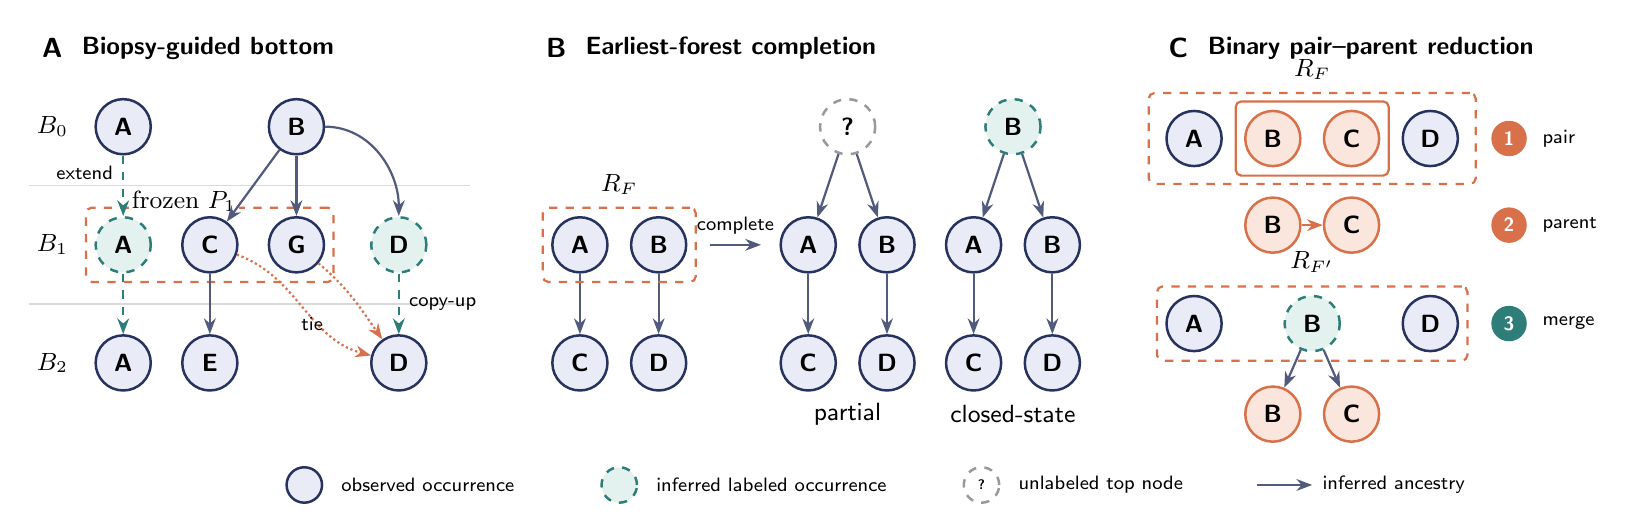
\begin{tikzpicture}

% ================= Panel A =================
\begin{scope}
  \node[badge] at (0,4) {A};
  \node[ttl] at (0.25,4) {Biopsy-guided bottom};

  \node[rowlab] at (0,3)   {$B_0$};
  \node[rowlab] at (0,1.5) {$B_1$};
  \node[rowlab] at (0,0)   {$B_2$};
  \draw[sep] (-0.3,2.25) -- (5.3,2.25);
  \draw[sep] (-0.3,0.75) -- (5.3,0.75);

  \node[obs] (A0) at (0.9,3)   {A};
  \node[obs] (B0) at (3.1,3)   {B};
  \node[inf] (A1) at (0.9,1.5) {A};
  \node[obs] (C1) at (2.0,1.5) {C};
  \node[obs] (G1) at (3.1,1.5) {G};
  \node[inf] (D1) at (4.4,1.5) {D};
  \node[obs] (A2) at (0.9,0)   {A};
  \node[obs] (E2) at (2.0,0)   {E};
  \node[obs] (D2) at (4.4,0)   {D};

  \node[box, fit=(A1)(C1)(G1)] (P1) {};
  \node[setlabel, fill=white, inner sep=1pt] at (1.67,2.05) {frozen $P_1$};

  \draw[infarr] (A0) -- (A1) node[pos=0.28, left, lbl=tl] {extend};
  \draw[arr] (B0) -- (C1);
  \draw[arr] (B0) -- (G1);
  \draw[arr] (B0) to[out=0,in=90] (D1);
  \draw[infarr] (A1) -- (A2);
  \draw[arr] (C1) -- (E2);
  \draw[infarr] (D1) -- (D2) node[midway, right, lbl=tl] {copy-up};
  \draw[tie] (C1) to[out=-20,in=165] (D2);
  \draw[tie] (G1) to[out=-40,in=125] (D2);
  \node[lbl=orng] at (3.3,0.5) {tie};

\end{scope}

% ================= Panel B =================
\begin{scope}[xshift=6.4cm]
  \node[badge] at (0,4) {B};
  \node[ttl] at (0.25,4) {Earliest-forest completion};

  % bottom forest
  \node[obs] (bA) at (0.3,1.5) {A};
  \node[obs] (bB) at (1.3,1.5) {B};
  \node[obs] (bC) at (0.3,0)   {C};
  \node[obs] (bD) at (1.3,0)   {D};
  \draw[arr] (bA) -- (bC);
  \draw[arr] (bB) -- (bD);
  \node[box, fit=(bA)(bB)] (RF) {};
  \node[lbl=orng, above=1pt of RF, font=\small] {$R_F$};

  \draw[arr] (1.95,1.5) -- (2.6,1.5) node[midway, above, lbl=navy] {complete};

  % partial
  \node[unl] (pT) at (3.7,3)   {?};
  \node[obs] (pA) at (3.2,1.5) {A};
  \node[obs] (pB) at (4.2,1.5) {B};
  \node[obs] (pC) at (3.2,0)   {C};
  \node[obs] (pD) at (4.2,0)   {D};
  \draw[arr] (pT) -- (pA); \draw[arr] (pT) -- (pB);
  \draw[arr] (pA) -- (pC); \draw[arr] (pB) -- (pD);
  \node[lbl=navy, font=\sffamily\small] at (3.7,-0.65) {partial};

  % closed-state
  \node[inf] (cT) at (5.8,3)   {B};
  \node[obs] (cA) at (5.3,1.5) {A};
  \node[obs] (cB) at (6.3,1.5) {B};
  \node[obs] (cC) at (5.3,0)   {C};
  \node[obs] (cD) at (6.3,0)   {D};
  \draw[arr] (cT) -- (cA); \draw[arr] (cT) -- (cB);
  \draw[arr] (cA) -- (cC); \draw[arr] (cB) -- (cD);
  \node[lbl=navy, font=\sffamily\small] at (5.8,-0.65) {closed-state};

\end{scope}

% ================= Panel C =================
\begin{scope}[xshift=14.3cm]
  \node[badge] at (0,4) {C};
  \node[ttl] at (0.25,4) {Binary pair--parent reduction};

  % 1: active component roots; existing descendant subtrees are omitted.
  \node[obs] (sA) at (0.2,2.85) {A};
  \node[hl]  (sB) at (1.2,2.85) {B};
  \node[hl]  (sC) at (2.2,2.85) {C};
  \node[obs] (sD) at (3.2,2.85) {D};
  \node[box, fit=(sA)(sB)(sC)(sD), inner sep=6pt] (rootsBefore) {};
  \node[setlabel, above=1pt of rootsBefore] {$R_F$};
  \node[box, draw=orng, solid, fit=(sB)(sC)] {};

  % 2: choose parent
  \node[hl] (qB) at (1.2,1.75) {B};
  \node[hl] (qC) at (2.2,1.75) {C};
  \draw[hlarr] (qB) -- (qC);

  % 3: merge
  \node[obs] (mA) at (0.2,0.5)  {A};
  \node[inf] (mB) at (1.7,0.5)  {B};
  \node[obs] (mD) at (3.2,0.5)  {D};
  \node[hl]  (mb) at (1.2,-0.65) {B};
  \node[hl]  (mc) at (2.2,-0.65) {C};
  \draw[arr] (mB) -- (mb); \draw[arr] (mB) -- (mc);
  \node[box, fit=(mA)(mB)(mD)] (rootsAfter) {};
  \node[setlabel, above=1pt of rootsAfter] {$R_{F'}$};

  % step badges
  \node[step=orng] (s1) at (4.2,2.85) {1}; \node[lbl=orng, right=2pt of s1] {pair};
  \node[step=orng] (s2) at (4.2,1.75) {2}; \node[lbl=orng, right=2pt of s2] {parent};
  \node[step=tl]   (s3) at (4.2,0.5)  {3}; \node[lbl=tl,   right=2pt of s3] {merge};

\end{scope}

% ================= Legend =================
\begin{scope}[yshift=-1.55cm, every node/.append style={font=\sffamily\scriptsize}]
  \node[obs, minimum size=4.5mm] (l1) at (3.2,0) {};
  \node[right=3pt of l1] {observed occurrence};
  \node[inf, minimum size=4.5mm] (l2) at (7.2,0) {};
  \node[right=3pt of l2] {inferred labeled occurrence};
  \node[unl, minimum size=4.5mm, font=\sffamily\bfseries\tiny] (l3) at (11.8,0) {?};
  \node[right=3pt of l3] {unlabeled top node};
  \draw[arr] (15.3,0) -- (16.0,0) node[right, text=black] {inferred ancestry};
\end{scope}

\end{tikzpicture}
\end{document}
